\section{辅助说明}

\subsection{运行方式}

\subsection{截图}

\begin{figure}[h!]
    \centering
    \begin{subfigure}{0.45\textwidth}
        \centering
        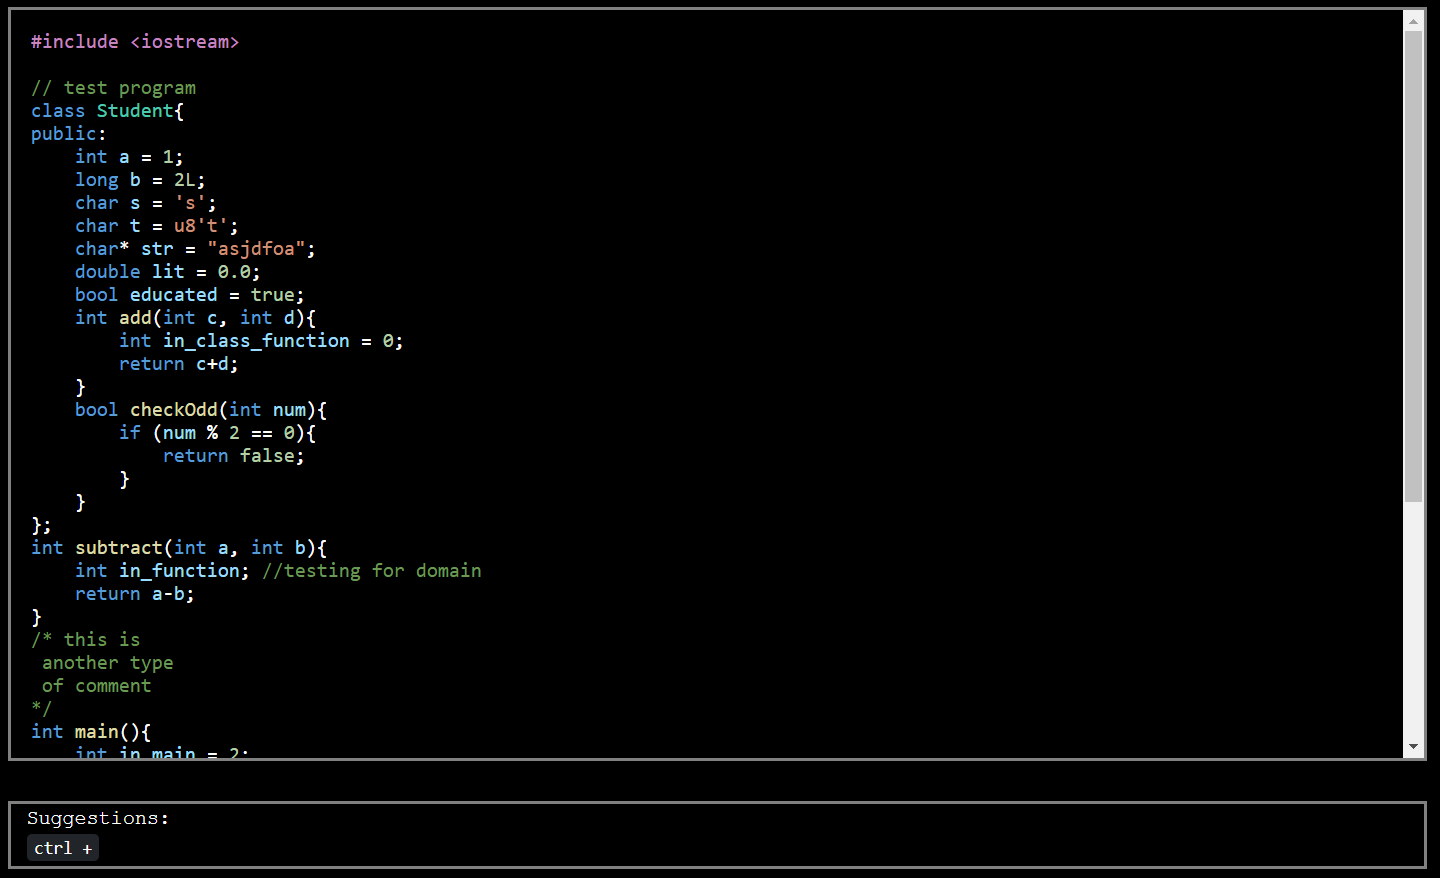
\includegraphics[width=\linewidth]{imgs/整体的样子.png}
        \caption{整体的样子}
        \label{fig:1}
    \end{subfigure}
    \hspace{1em}
    \begin{subfigure}{0.45\linewidth}
        \centering
        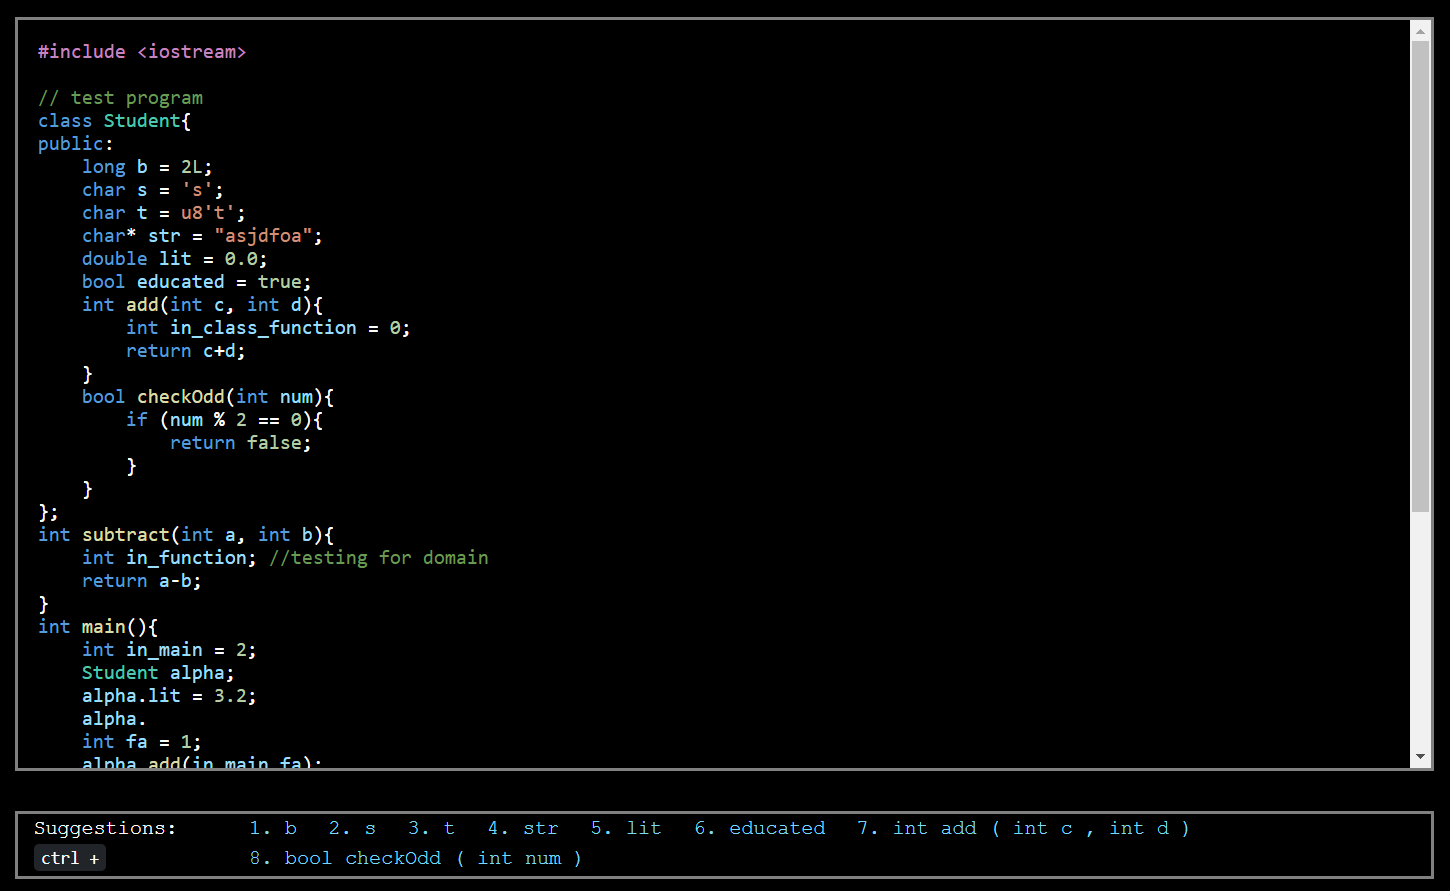
\includegraphics[width=\linewidth]{imgs/类成员对象和成员函数补全.png}
        \caption{类成员对象和成员函数补全}
        \label{fig:2}
    \end{subfigure}
    \begin{subfigure}{0.45\textwidth}
        \centering
        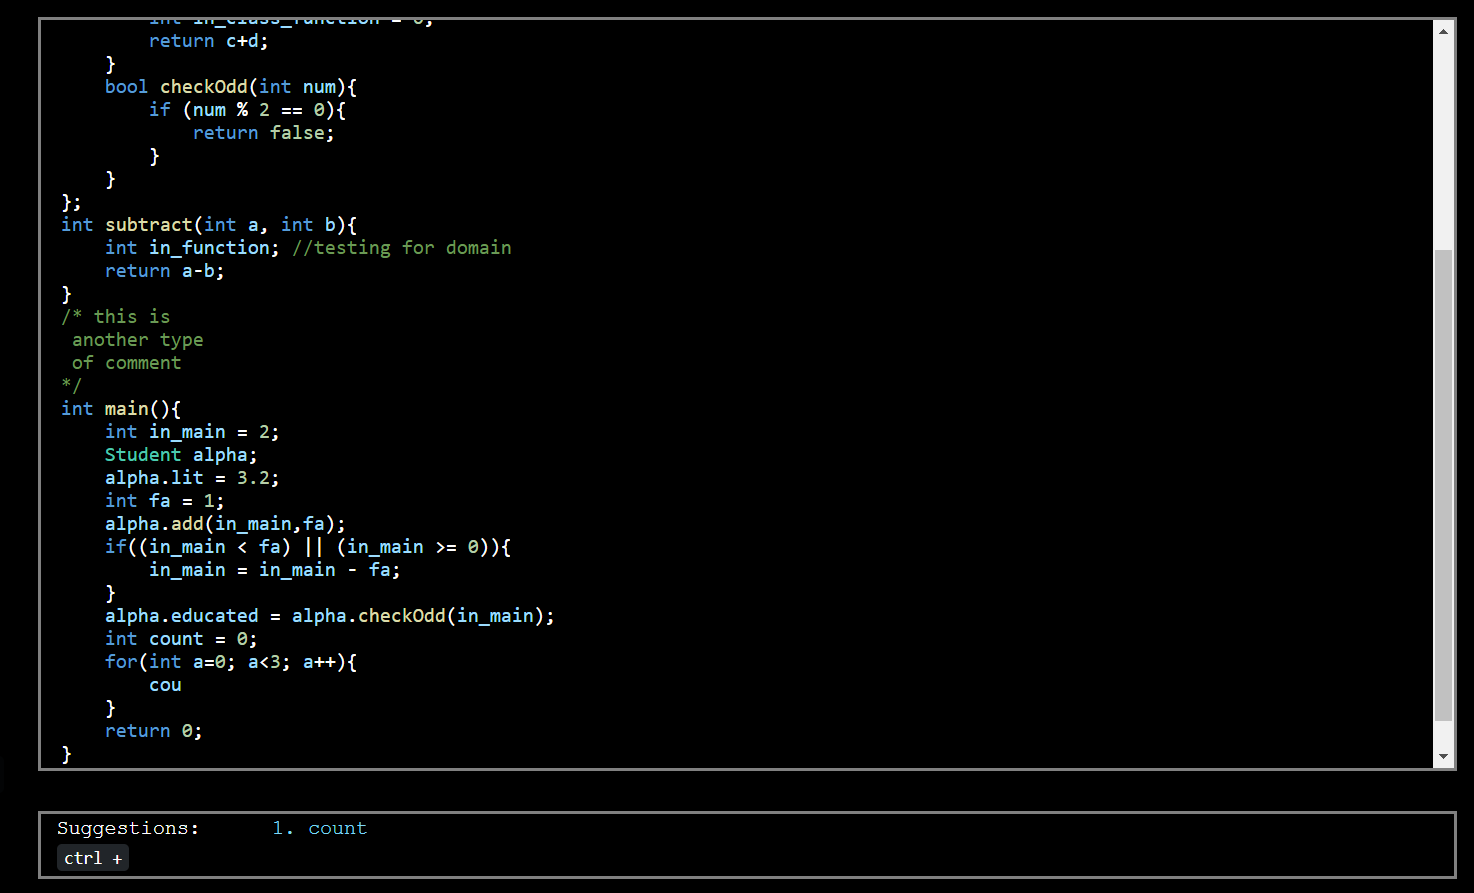
\includegraphics[width=\linewidth]{imgs/定义域内变量补全.png}
        \caption{定义域内变量补全}
        \label{fig:3}
    \end{subfigure}
    \hspace{1em}
    \begin{subfigure}{0.45\linewidth}
        \centering
        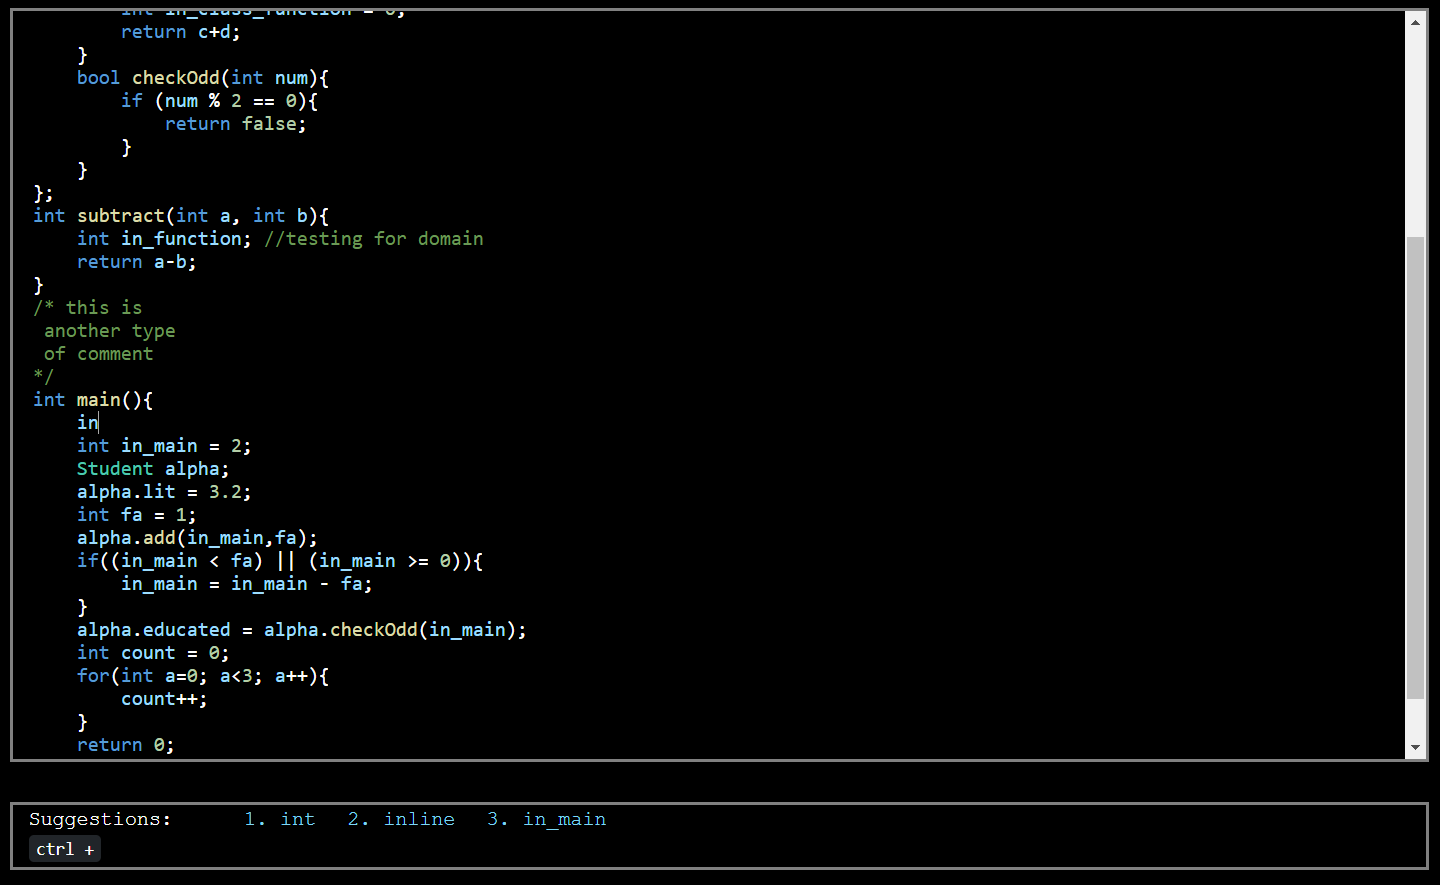
\includegraphics[width=\linewidth]{imgs/非定义域内变量(in_function)不补全.png}
        \caption{非定义域内变量不补全}
        \label{fig:4}
    \end{subfigure}
    \caption{代码高亮与提示程序截图}
\end{figure}

a: 图(a)是代码高亮和补全程序的一个基本页面展示。当用户输入代码时,输入的代码会根据相应类型进行颜色的变换(高亮),如class是亮绿色,#include是粉紫色等等。

b: 对于类的成员变量和成员函数,只会在用户在对应的类对象后输入"."或者"->",相应的成员函数和变量会在suggestions中提示。用户可以通过ctrl+显示按键的方式,对代码进行补全,如图(b)所示。

c: 图(c)展示了程序中实现了对定义域(或者说可调用域)和可操作域的实现。当函数或者是变量被定义或者声明后,用户再次在相同定义域domain中试图输入时,会有提示和补全信息。


d: 而对于有着特定定义域的变量来说,它们不会在除自身可用定义域以外的其他定义域中被提示可补全,如图(d)中的in_function。